\begin{flushright}
	
\end{flushright}\chapter{Literature Review}
\label{cha:2_literature}
\parskip=0ex

\section{Introduction to ASL}
\label{sec:1_intro}
In the early of 1800s, the population of deaf Americans was only about a few thousand. The Deaf communities made various signing systems and at that time, there was no standard sign language existed. These situasion are now called as an Old American Sign Language. The current used American Sign Language is actually related to this language~\cite{startAslCom}.

The beginning of the current used American Sign Language was started in 1814 with Dr. Thomas Hopkins Gallaudet, a minister from Hartford, Connecticut. The neighbor of him, named Mason Fitch Cogswell, had a nine years old deaf daughter, Alice Cogswell. Although Alice could not speak or hear, Dr. Gallaudet found that she was very smart, so that he wanted to teach her how to communicate. He then had a little success in making Alice enabled to read and spell, but he felt the method he used to teach was not effective. Therefore, Dr. Gallaudet gained a community support and money to go to Europe, in order to learn the best educational methods for the deaf, since there was a history of deaf education in Europe.

Arrived at Europe, Gallaudet met three other figures, Abbe Sicard, Jean Massieu, and Laurent Clerc. Sicard was a successor of Abbe de l'Epee's at the National Insitute for Deaf-Mutes. The other two learned the deaf education from Sicard and became expert deaf educators. Gallaudet then learned how to teach the deaf from these instructors and yet he took private lessons with Clerc, the one of the best teachers at the institute.

After accomplished the study, Gallauded travelled back to America, accompanied by Clerc. He proposed to Clerc to join him because he knew Clerk would be a huge help in starting a school for the deaf, which is now known as the American School for the Deaf. This school was established in Gallaudet hometown, Hartford, in 1817 as the first public free deaf school in the U.S~\cite{wiki:xxx}. At this point, Gallaudet and Clerc had successfully make a huge milestone in American Deaf history.

The name of the school was quickly spread around the U.S., making deaf students all over the country came together to study in this school. Just like the school in Europe, the students also brought their own local sign language to the school. American Sign Language derived from these signs and from French Sign Language that was learned from Clerc. Gallaudet retired in 1830, but the taught for the deaf was still continued by Clerc until the 1850s. By 1863, there were twenty two deaf schools in the U.S and most of them were founded by Clerc's students. The school founded by Clerc's students continued to use Clerc's deaf education methods.

After Thomas Hopkins Gallaudet passed away in 1851, his youngest son, Edward Miner Gallaudet continued the work of him in deaf education. Edward then became a teacher at his father's school and in 1857, he was asked to be the headmaster of the Columbia Insitution for the Deaf and Dumb and the Blind in Washington, D.C. Edward also had a big role in deaf education since he presented an idea to provide a deaf college to Congress and in 1864, the permit to issue a college degrees for Columbia Insitute was passed. In 1864, the Columbia Insitute's first college division for the deaf named the National Deaf-Mute College was opened. The college was renamed to Gallaudet College tributed to Thomas Hopkins Gallaudet. Later in 1986, it was renamed to Gallaudet University, and it is known today as the first and only deaf univerity in the world.

The other schools spreaded around the U.S also took roles to pass down their education from the American School for the Deaf to the next generation of deaf students the contact language that has known as today's American Sign Language. In 1900s, the nationwide network of deaf schools was completed. The community were given the opportunity to be with other deaf to share their sign language and cultural experiences without any communication barriers. The American Sign Language used today is a result of almost two hundred years of deaf people passing down their language from one to another generation that now become one of the most used languages in the U.S~\cite{dawnSignPress}.

\section{Previous 3D Based text to ASL system}
\label{sec:2_3dBased}

\section{ASL Lexicon Video Dataset}
\label{sec:3_ASLDataset}
The American Sign Language Lexicon Video Dataset~\cite{ASLLexiconVideoDataset} was made primarily to provide a dictionary of Sign Language. Usually when we face an English word that we do not know, we will look it up in a dictionary. But, when an American Sign Language user encounters an unknown sign, the media for s/he to look it up is very limited.

The ASL Lexicon Video Dataset is a public dataset which contains thousands of distinct ASL signs in the form of high-quality video sequences. This dataset was made as a part of a project to provide a vision-based system used to look up the meaning of an ASL sign. The main part of this collection is its comprehenssiveness. Some approaches to recognize signs in a vision-based manner only could cover small vocabularies (20-300 signs) and often rely on color markers~\cite{vision1},~\cite{vision2}. Therefore, this dataset was hoped to be able to make a trend for developing vision-based methods that operate on markerless images and can cover a broader vocabulary.

\begin{figure}[H]
	\begin{center}
		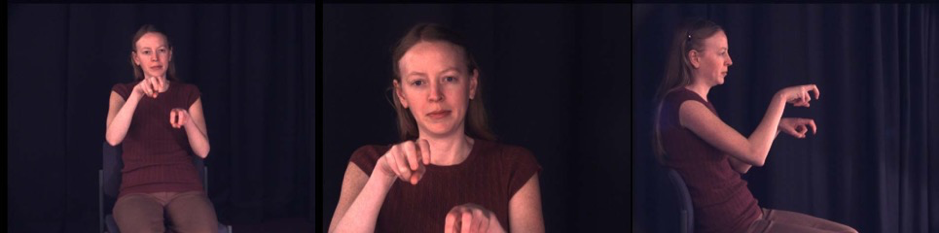
\includegraphics[width=1.0\textwidth]{figures/asl_4_side.png}
		\caption{One of the ASL Lexicon Dataset frontal views (left), the face view (middle), and the side view (right), for a frame in a video sequence~\cite{ASLLexiconVideoDataset}.} 
		\label{fig:1_ASLView}
	\end{center}
\end{figure}

The total number of signs contained in the dataset has a similar scale and scope with the existing English-to-ASL dictionaries~\cite{gallaudetBook1},\cite{gallaudetBook2}. This dataset has at least one sign example figured by a native signer, for almost about 3,000 sign contained in the Gallaudet Dictionary of American Sign Language~\cite{gallaudetBook2}.

Usually for their communication, ASL users sometimes spell out English words using the alphabet. Along with the existing dataset~\cite{gallaudetBook1},~\cite{gallaudetBook2}, in The ASL Lexicon Video dataset, the fingerspelled signs were not included, as they were counted as "loan signs".

In the described dataset, each sign was performed by native ASL signers. The number of involved native ASL users for this dataset was four people. The video sequences were collected using a four-camera system that concurrently captured two-frontal views, one side view and one view zoomed in on the face of the signer. For the side view and the two frontal views, the upper body took over a relatively large part of the scene frames. For the face view, the frontal view of the face which took over the large part of the scene frames. All video sequences were recorded and provided in color.

The video of the side view, the first frontal view, and the face view was captured at 60 frames per second, and each frame has a resolution of 640x480 pixels. Then, for the video of the second frontal view, it was captured at 30 frames per second with a resolution of 1600x1200 pixels per frame. The second frontal view was purposely made to facilitate a more detail display of the hands, compared to the 640x480 views.

The dataset were stored in a lossless compression format and it can be read using a C++ code provided on the official website. A compressed QuickTime version of video sequences was also created, with purpose to enable the viewers to quickly browse the video.

\begin{figure}[H]
	\begin{center}
		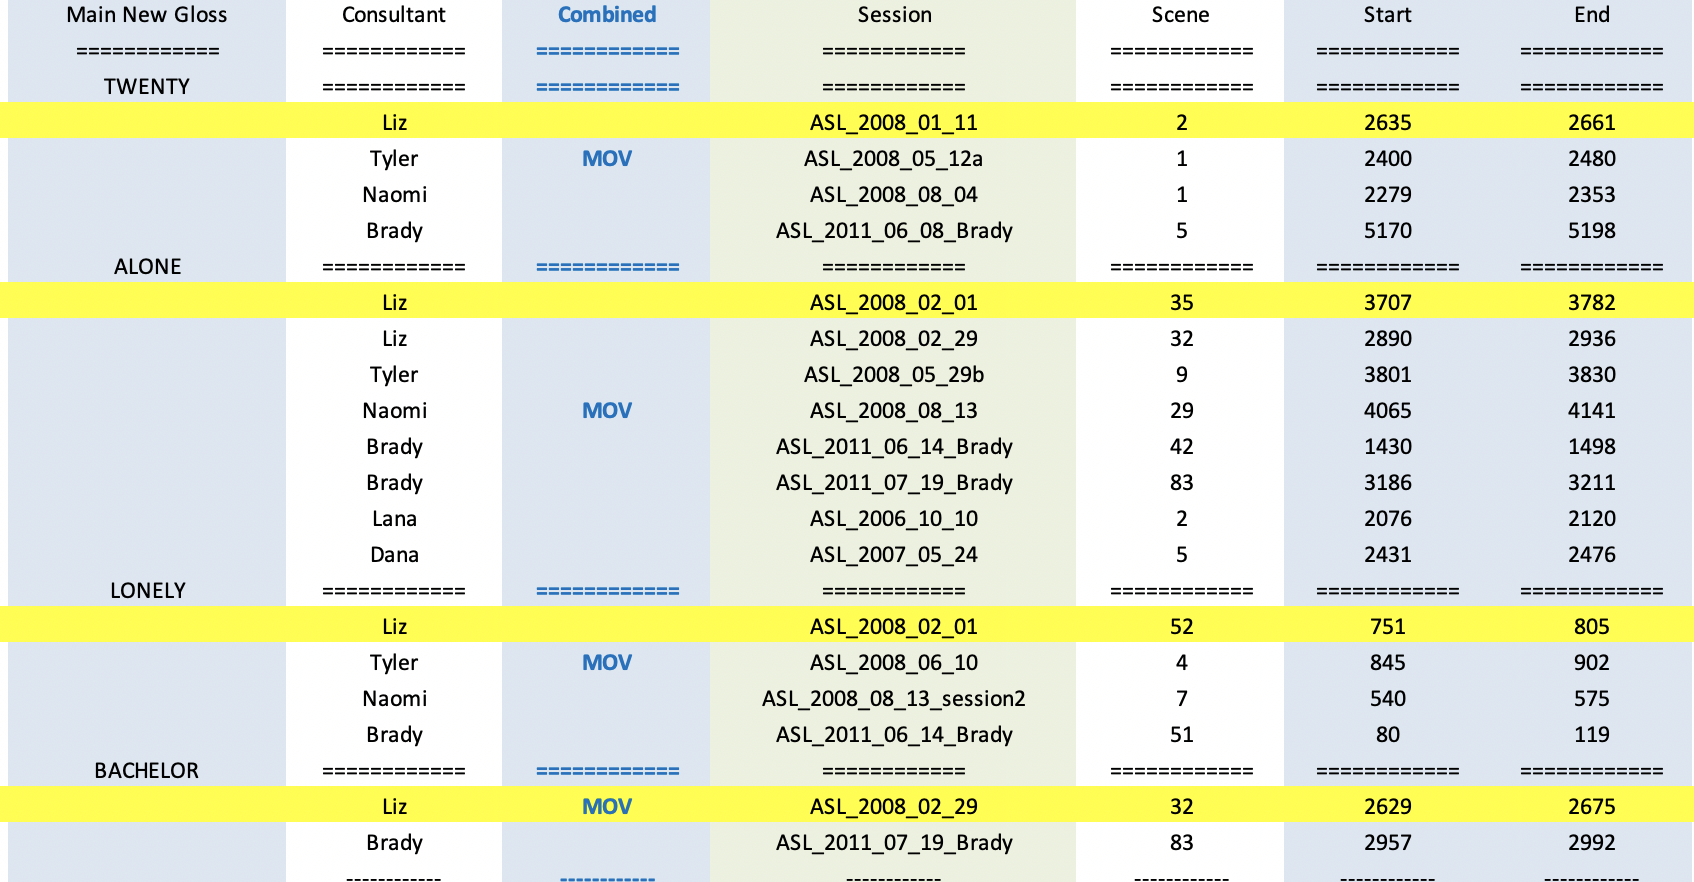
\includegraphics[width=1.0\textwidth]{figures/excelASLDataset.png}
		\caption{Annotation of ASL Lexicon Video Dataset. Retrieved from the annotation file of~\cite{ASLLexiconVideoDataset}.} 
		\label{fig:2_ASLAnnotation}
	\end{center}
\end{figure}

An excel file showing the annotation was also provided. Since ASL signs have no written form, so the class label for each sign were written in an approximated English, called a "gloss". A gloss could possibly assign to two different signs if they corresponded to the same ASL Lexical item.

A video sequence was stored multiple signs. For each sign in a video sequence, the annotation was written its start and end frames, the gloss, whether the sign is one-handed or two-handed, and a signer ID. The signer IDs were written to allow researchers to do experiments for user-dependent and user-independent sign recognition.

\section{OpenPose}
\label{sec:4_openpose}
OpenPose~\cite{cao2018openpose} is an open library to detect multi-person pose estimation. It was claimed as the first bottom-up representation of association scores using a set of 2D vector fields that encode the location and orientation of limbs shown on the image domain, named Part Affinity Fields.

\begin{figure}[H]
	\begin{center}
		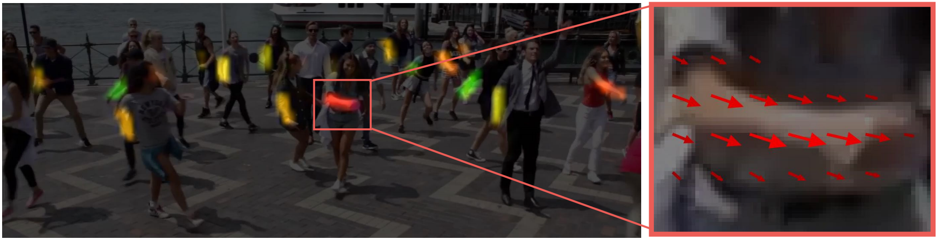
\includegraphics[width=1.0\textwidth]{figures/paf.png}
		\caption{Left: Part Affinity Fields corresponding to the limb that connected elbow and wrist. Right: a 2D vector in each pixel of every PAF which encoded the position and orientation of the limbs~\cite{cao2018openpose}.} 
		\label{fig:3_OpenPose}
	\end{center}
\end{figure}

This research had some improvements compared to its previous version~\cite{cao2017realtime}. From this newer version of work, Cao et. al proved that to achieve a maximum accuracy, the most important part in the work is to refine the Part Affinity Fields, while ignoring the body part prediction refinement. The first body and food keypoint detector combination was also propposed in this research, created based on foot dataset annotation that will be publicly released. The OpenPose was claimed as the first open source library which able to detect 2D multi-person pose, including the body, foot, hand, and facial keypoints, in a realtime manner.

\begin{figure}[H]
	\begin{center}
		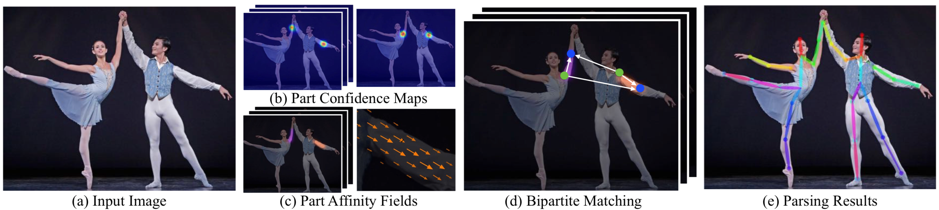
\includegraphics[width=1.0\textwidth]{figures/openposesystem.png}
		\caption{Overall system flow. (a) Entire image is taken as the input for a CNN to predict the join (b)confidence maps for body part is detected (c) detection of PAFs (d) bipartite matching to associate body part candidates (e) assembly of PAFs into full body poses for all detected people in the image~\cite{cao2018openpose}.} 
		\label{fig:4_OpenPoseFlow}
	\end{center}
\end{figure}

The OpenPose overall system can be seen at Fig. 2.4. The input is a color image (Fis. 2.4a) and the output is the 2D locations of the anatomical keypoints for each person in the image (Fig. 2.4e). The input image, firstly is forwarded to a feedforward network to predict a set of 2D confidence maps of body part locations (Fig. 2.4b), and a set of 2D vector PAFs (Fig. 2.4c), which encode the association degree between body parts. Lastly, greedy inference (Fig. 2.4d) will parse the confidence maps and the affinity fields to output the 2D keypoints for all people in the input image.

Compared to the existing 2D body pose estimation libraries, such as Mask R-CNN or Alpha-Pose, OpenPose has many superiorities. The existing libraries require the users to implement most of their pipeline, provide their own frame reader, a media to display the results, and provide the file generation for storing the results in JSON or XML, etc. The existing facial and body keypoint detectors are also not combined, so different libraries are required for each purpose. Different from the mentioned works, OpenPose can overcome all of the problems. It is able to be run on many different platforms, such as, Ubuntu, Windows, Mac OSX, and embedded systems. Different hardware, such as CUDA GPUs, OpenCL GPUs, and CPU only devices are also supported by this framework. The input types, images, video, webcam, and IP camera streaming are also served to be chosen by the user. The users can also select to display the results or save them on the disk. They can also choose which part of the human body they want to detect. Pixel coordinate normalization, number of GPUs to be used and frames skipping options are also the superiorities of this library.

\begin{figure}[H]
	\begin{center}
		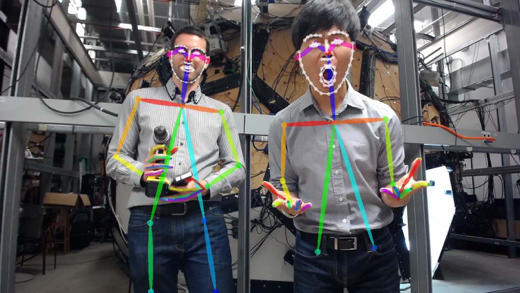
\includegraphics[width=0.8\textwidth]{figures/openposeeg.png}
		\caption{Output of OpenPose, body, foot, hand, and facial keypoints are detected in a real-time manner.~\cite{cao2018openpose}.} 
		\label{fig:4_OpenPoseFlow}
	\end{center}
\end{figure}